\section{Ручное тестирование системы}

\subsection{Тестирование отказоустойчивости}

Проверка корректности реализации алгоритма Raft проводилась с использованием
ручных интеграционных испытаний. Для этого на локальной машине было запущено
три экземпляра Raft-узлов, каждый из которых инициализировался собственной
конфигурацией и прослушивал уникальный TCP-порт. На этапе инициализации узлы
формируют сетевые потоки (\texttt{peer threads}), регистрируют gRPC-сервисы и
начинают обмен heartbeat-сообщениями.

В первом эксперименте система демонстрирует штатное избрание лидера:
через заданный таймаут по истечении срока аренды один из узлов инициировал
выборы (лог содержит сообщение \texttt{Starting election in term 1}) и,
получив кворум голосов, объявил себя лидером (\texttt{I'm the leader now}).
В таком состоянии кластер готов принимать клиентские запросы, а
закоммиченные записи будут реплицироваться на оставшиеся узлы. Лог мастера
изображен на рис.~\ref{fig:leader_log}. Лог одной из реплик же представлен
на рис.~\ref{fig:replica_log}.

\begin{figure}
  \centering
  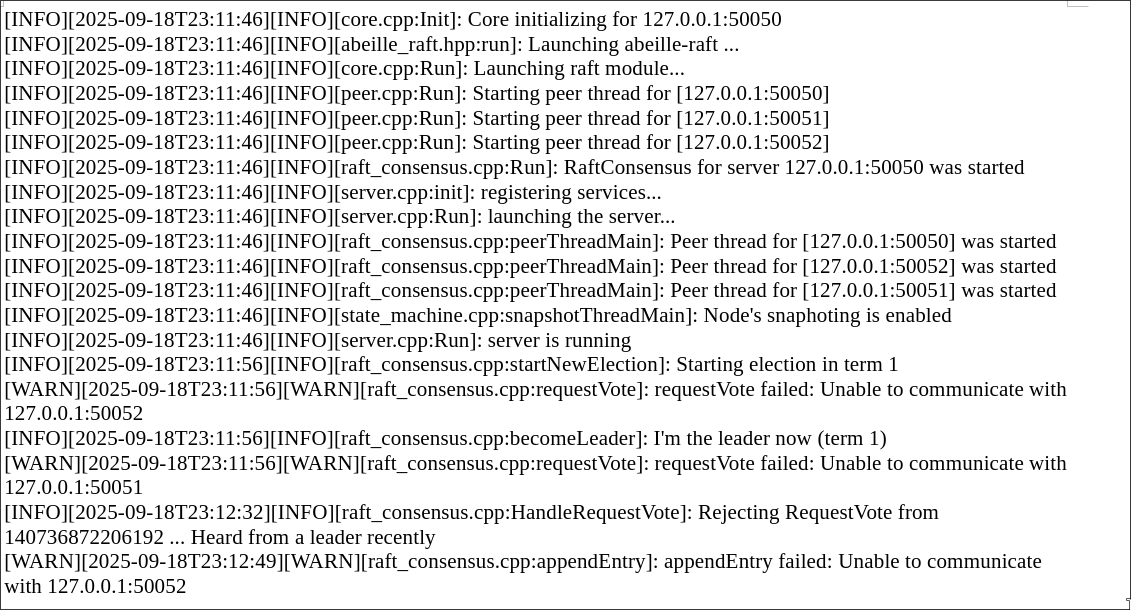
\includegraphics[scale=0.4]{inc/leader-log.png}
  \caption{Лог мастера при первом выборе лидера}
  \label{fig:leader_log}
\end{figure}

\begin{figure}
  \centering
  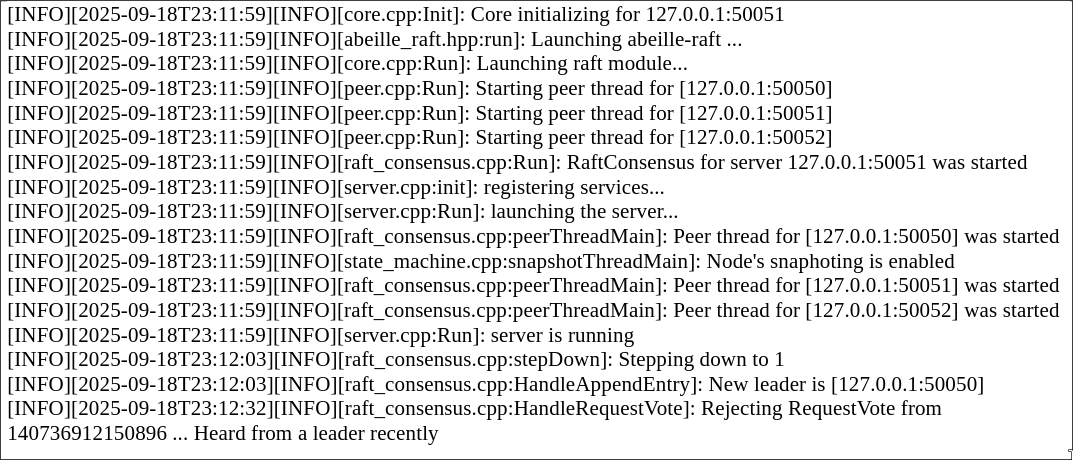
\includegraphics[scale=0.4]{inc/replica-log.png}
  \caption{Лог реплики при первом выборе лидера}
  \label{fig:replica_log}
\end{figure}

Затем моделировался отказ лидера: первый узел был остановлен, что привело к
прекращению рассылки heartbeat-пакетов (см. рис.~\ref{fig:leader-shutdown}).

\begin{figure}
  \centering
  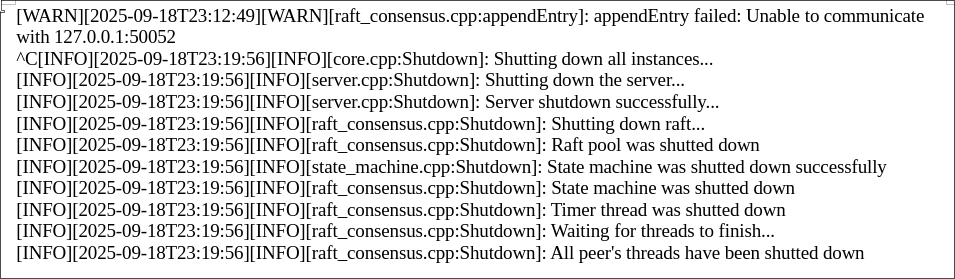
\includegraphics[scale=0.4]{inc/master-after-shutdown.png}
  \caption{Логи при остановке мастера}
  \label{fig:leader-shutdown}
\end{figure}

Спустя период \texttt{election timeout} один из оставшихся узлов инициировал
новый раунд выборов (терм 2), получил поддержку большинства и стал новым
лидером. В логах зафиксировано событие \texttt{becomeLeader} с указанием нового
терма, что подтверждает корректную работу механизма смены лидерства и
сохранение согласованности состояния кластера, это представлено на рис.
~\ref{fig:new-master}.

\begin{figure}
  \centering
  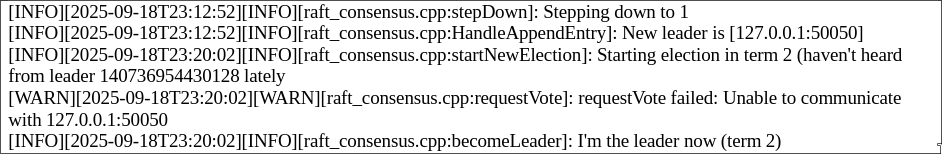
\includegraphics[scale=0.4]{inc/replica-master-after-shutdown.png}
  \caption{Логи нового мастера после остановки старого}
  \label{fig:new-master}
\end{figure}

Процесс голосования реплики за нового лидера представлен на рис.
~\ref{fig:replica-after-new-leader}.

\begin{figure}
  \centering
  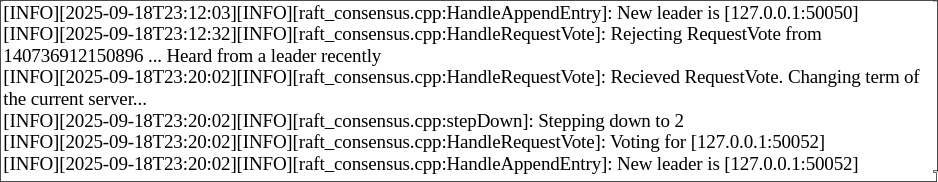
\includegraphics[scale=0.4]{inc/replica-after-shutdown.png}
  \caption{Процесс голосования за нового лидера}
  \label{fig:replica-after-new-leader}
\end{figure}

Такие испытания позволяют убедиться, что система корректно реагирует на сбои:
потеря лидера не приводит к недоступности сервиса, а лишь инициирует повторные
выборы, после которых кластер восстанавливает способность обрабатывать запросы.
В сочетании с механикой репликации и commit-индексов это гарантирует, что все
закоммиченные записи остаются видимыми для клиента даже при перезапуске узлов.

\subsection{Инициализация клиентского приложения и подключение к кластеру}

Тестирование вычислительного процесса начинается с запуска консольного клиента
с указанием конфигурационных файлов пользователя и кластера. На
рис.~\ref{fig:client_start} приведён фрагмент журнала запуска клиента. В ходе
подключения клиент последовательно обходит адреса, указанные в
\texttt{client\_config.json}. Поскольку первый узел кластера
(\texttt{127.0.0.1:50050}) в момент запуска был недоступен, попытка
установления соединения завершилась ошибкой, что зафиксировано в логах с
уровнем \texttt{ERROR}. После истечения интервала переподключения клиент
автоматически переходит к следующему адресу и успешно устанавливает соединение
с узлом \texttt{127.0.0.1:50051}, а затем и с \texttt{127.0.0.1:50052}. Такая
стратегия повышает отказоустойчивость системы: пользователь не обязан вручную
выбирать рабочий узел, так как клиент сам находит доступного участника
кластера.

\begin{figure}[h!]
    \centering
    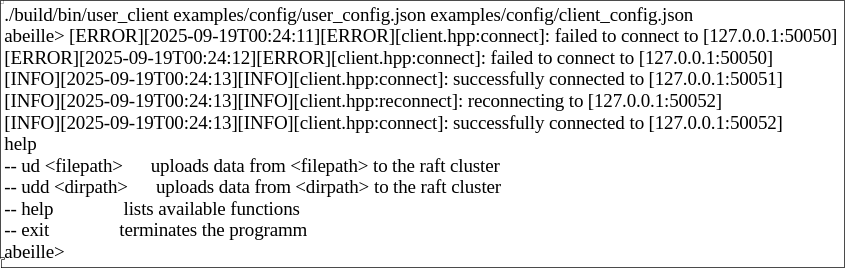
\includegraphics[width=0.8\linewidth]{inc/client-shell.png}
    \caption{Журнал запуска клиентского приложения: обработка недоступности узла и
    успешное подключение к кластеру.}
    \label{fig:client_start}
\end{figure}

После установления соединения клиент переходит в интерактивный режим, предлагая
пользователю список доступных команд. В частности, доступны функции загрузки
данных из файла или директории (\texttt{ud}, \texttt{udd}), вывод справочной
информации и завершение работы программы. На этом этапе система готова к
приёму задания и дальнейшему тестированию логики репликации и обработки задач.

\subsection{Запуск вычислительных узлов и их подключение к кластеру}

После инициализации клиентской части производится запуск вычислительных узлов,
которые будут непосредственно выполнять задачи.Логи на
рис.~\ref{fig:worker_start} демонстрируют, что, как и в случае с клиентом,
воркер поочерёдно пытается подключиться к указанным в
\texttt{client\_config.json} узлам. Первая пара попыток к
\texttt{127.0.0.1:50050} завершилась ошибкой соединения, после чего воркер
переключился на следующий адрес и успешно установил потоковое RPC-соединение с
\texttt{127.0.0.1:50051}, а затем и с лидером \texttt{127.0.0.1:50052}.

\begin{figure}[h!]
    \centering
    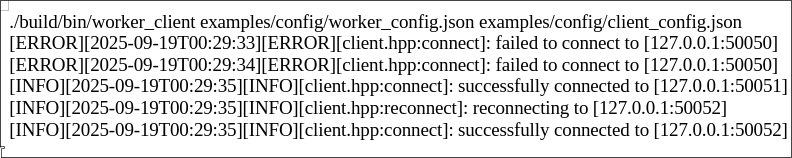
\includegraphics[width=0.8\linewidth]{inc/worker-log.png}
    \caption{Логи запуска вычислительного узла: автоматический обход узлов и успешное подключение.}
    \label{fig:worker_start}
\end{figure}

После установления соединения воркер переходит в состояние \texttt{IDLE},
публикуя свой статус в поток \texttt{WorkerService.Connect}, что позволяет
кластеру учитывать его при назначении новых задач. Таким образом, уже на этом
этапе проверяется важная функциональность системы — автоматический выбор
доступного узла и готовность воркера принимать задания от лидера кластера.

\subsection{Тестирование выполнения задания}

Для проверки корректности работы системы был проведён end-to-end тест с
использованием простого вычислительного задания. В качестве тестовой функции
был выбран алгоритм факторизации числа на простые множители, реализованный на
C++. Такая задача является хорошим примером для функционального тестирования:
она не требует сложной подготовки данных, но даёт детерминированный и легко
проверяемый результат. Код задания представлен в приложении В. В качестве
входных данных подавались 10000 чисел.

Постановка задачи выполнялась из интерактивной консоли клиентского приложения с
помощью команды \texttt{ud}, передающей содержимое \texttt{data.json} в
кластер. Это представлено на рис.~\ref{fig:client-send}. Клиент подтвердил
успешную загрузку данных, а после обработки задачи вывел сообщение о получении
результата.

\begin{figure}[h!]
    \centering
    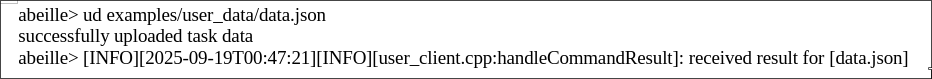
\includegraphics[width=0.8\linewidth]{inc/client-send.png}
    \caption{Процесс пересылки данных на клиенте}
    \label{fig:client-send}
\end{figure}

На стороне лидера Raft логи показан полный путь задачи: назначение её
конкретному воркеру, репликацию соответствующей команды в Raft-лог, достижение
кворума и коммит, а также последующую фиксацию результата (см.
рис.~\ref{fig:master-log-task}). При этом реплика синхронизировалась с лидером,
что видно по сообщениям \texttt{HandleAppendEntry} и обновлению индексов
коммита (см. рис.~\ref{fig:replica-log-task}).

\begin{figure}[h!]
    \centering
    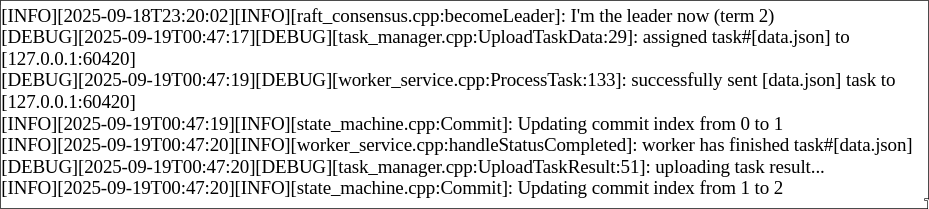
\includegraphics[width=0.8\linewidth]{inc/master-log-task.png}
    \caption{Лог мастера при назначении задания}
    \label{fig:master-log-task}
\end{figure}

\begin{figure}[h!]
    \centering
    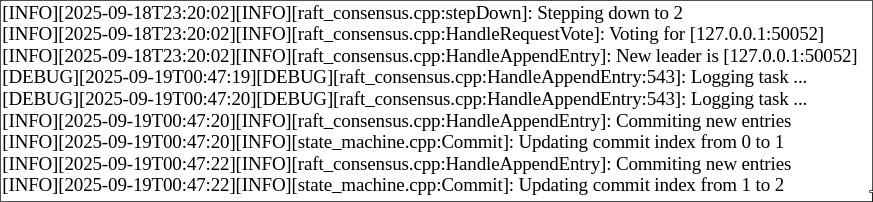
\includegraphics[width=0.8\linewidth]{inc/replica-log-task.png}
    \caption{Лог реплики при назначении задания}
    \label{fig:replica-log-task}
\end{figure}

Логи вычислительного узла подтвердили успешное получение задания: воркер перешёл
в состояние \texttt{BUSY}, инициировал локальный процесс обработки данных
через IPC, корректно завершил вычисление и вернул результат обратно в кластер
(см. рис.~\ref{fig:worker-log-task}).

\begin{figure}[h!]
    \centering
    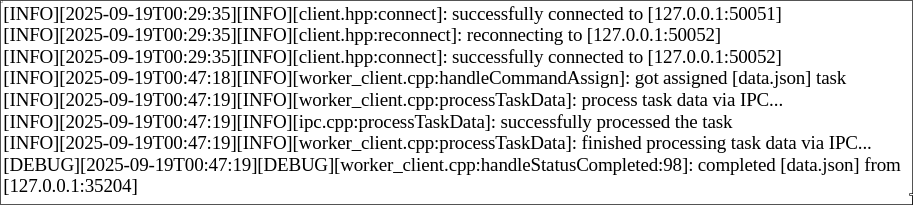
\includegraphics[width=0.8\linewidth]{inc/worker-log-task.png}
    \caption{Лог вычислительного узла при выполнении работы}
    \label{fig:worker-log-task}
\end{figure}

На стороне мастера была зафиксирована команда \texttt{RAFT\_COMMAND\_MOVE},
переведшая задачу в статус завершённой, после чего результат был передан
пользовательскому клиенту. Таким образом, в рамках теста была проверена вся
цепочка обработки: от приёма входных данных до финализации состояния в машине
состояний и возврата результата.

Проведённый эксперимент подтверждает корректность реализации основных
механизмов системы: клиентские запросы реплицируются и коммитятся только при
достижении кворума, воркеры получают задачи и публикуют статус их выполнения,
а пользователь всегда наблюдает согласованное состояние кластера, даже при
ранее проведённых сменах лидера или мертвых узлах.

\subsection{Нагрузочный тест с 50 параллельными клиентами}

Для проверки поведения системы при высокой конкурентной нагрузке был
организован сценарий с одновременной работой пятидесяти клиентских процессов.
Каждый клиент открывал двунаправленное gRPC-соединение с кластером, отправлял
одну команду \texttt{ud} для постановки задачи в очередь и завершал работу,
освобождая слот для следующих запусков. Параллельный запуск был реализован
средствами утилиты \texttt{GNU parallel} (см. рис.~\ref{fig:leader-multi-conn}),
обеспечивающей одновременный запуск 50 процессов с минимальной задержкой между
стартами.

\begin{figure}[h!]
    \centering
    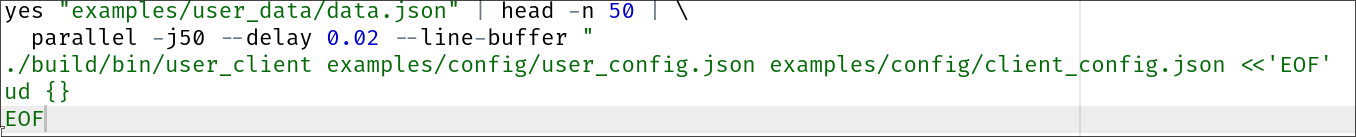
\includegraphics[width=0.95\linewidth]{inc/load-multi.png}
    \caption{Нагрузочный тест}
    \label{fig:leader-multi-conn}
\end{figure}

В данном тесте использовались два рабочих узла (воркера). Кластер Raft выбрал
лидера в начале прогона, после чего последовательно обрабатывал поступающие
задания. В журнале лидера наблюдается монотонное увеличение индекса коммита
каждой новой записи лога (рис.~\ref{fig:leader_log_50}), что подтверждает
корректную репликацию команд и достижение кворума. Каждое успешно завершённое
задание сопровождается сообщением
\texttt{worker\_service.cpp:handleStatusCompleted}, после чего в машине
состояний фиксируется переход задачи из состояния \texttt{assigned} в
\texttt{completed}.

\begin{figure}[h!]
    \centering
    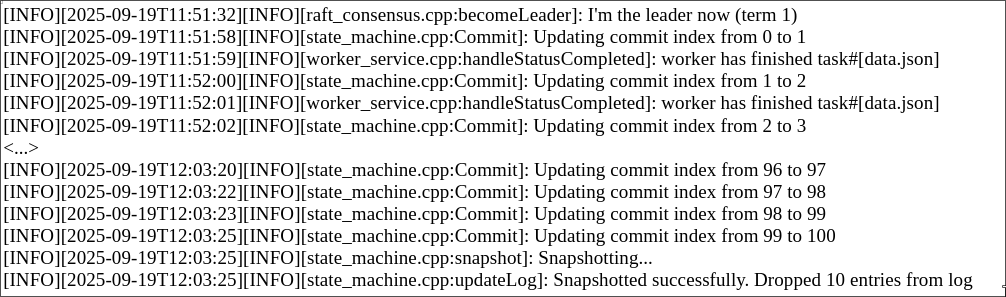
\includegraphics[width=0.95\linewidth]{inc/leader-multi-conn.png}
    \caption{Фрагмент лога лидера во время нагрузочного теста с 50 клиентами}
    \label{fig:leader_log_50}
\end{figure}

При достижении сотого коммита сработал механизм создания снепшота, что
подтверждается сообщением \texttt{Snapshotting...} в логах. После успешного
сохранения состояния машины состояний на диск (\texttt{Snapshotted
successfully}) из лога были удалены 10 записей, как и предусмотрено параметром
\texttt{snapshot\_after} в конфигурации. Продолжение работы кластера после
создания снепшота не вызвало увеличения задержек или ошибок репликации, что
свидетельствует о корректности реализации механизма архивации и его
прозрачности для клиентских приложений.

Таким образом, тест показал, что система способна обрабатывать десятки
одновременных подключений, сохраняя линейризуемость состояния и выполняя
своевременное архивирование лога без нарушения доступности сервиса.

\subsection{Тестирование на задаче с большим объёмом данных}

Для проверки корректности работы системы при выполнении ресурсоёмких задач был
проведён эксперимент с входными данными увеличенного размера (около двух
миллионов элементов). Задача была отправлена в кластер с использованием
стандартного клиента и поступила на один из доступных рабочих узлов. Фрагмент
лога воркера приведён на рис.~\ref{fig:worker_bigdata}.

\begin{figure}[h!]
    \centering
    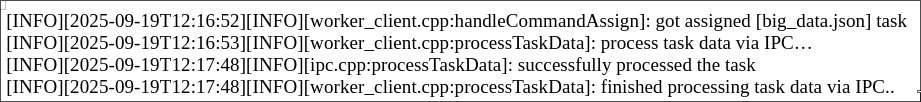
\includegraphics[width=0.95\linewidth]{inc/worker-big-data.png}
    \caption{Лог вычислительного узла при обработке задачи с 2 млн элементов}
    \label{fig:worker_bigdata}
\end{figure}

Как видно из лога, узел получил команду назначения задачи
(\texttt{handleCommandAssign}), после чего перешёл к фазе обработки данных через
IPC-механизм (\texttt{processTaskData}). Общая длительность обработки составила
около 56 секунд, что соответствует ожидаемому времени выполнения для задачи
данного объёма. По завершении вычислений задача была успешно отмечена как
выполненная (\texttt{finished processing task data via IPC}), а результат был
передан обратно в кластер и зафиксирован в машине состояний.

Данный эксперимент подтвердил, что система корректно обрабатывает задачи
увеличенной сложности и объёма, при этом не теряя связи с кластером и
сохраняя линейризуемость состояния. В течение всего времени выполнения других
ошибок или повторных назначений задачи не наблюдалось, что демонстрирует
устойчивость и надёжность реализации даже при продолжительных вычислениях.
